\chapter{Code generation and the Build process}
\label{cha:code-generation}

This chapter describes in detail the automatic generation of the
configuration code for \ee\ and the build process of an \ee\
application. The process of automatic generation of the configuration
code is the method used by \rtd\ to generate \ee\ configuration code
starting from an OIL configuration file. The Build Process is the set
of operations that are used to compile the application source code
together with the configuration source code.

Code Generation and Build Process need to be performed in two separate
stages. Each stage can be enabled or disabled by acting on the project
properties. To open the Project properties, right click on the project
name in the navigation toolbar, and then select ``Properties'', as
shown in Figure \ref{fig:build1}. After that, you can select
``Builders'' in the left list, and activate only the desired subset of
the build process. Please note, that all checkboxes are typically
checked, as shown in Figure \ref{fig:build2}.

\begin{figure}
  \begin{center}
    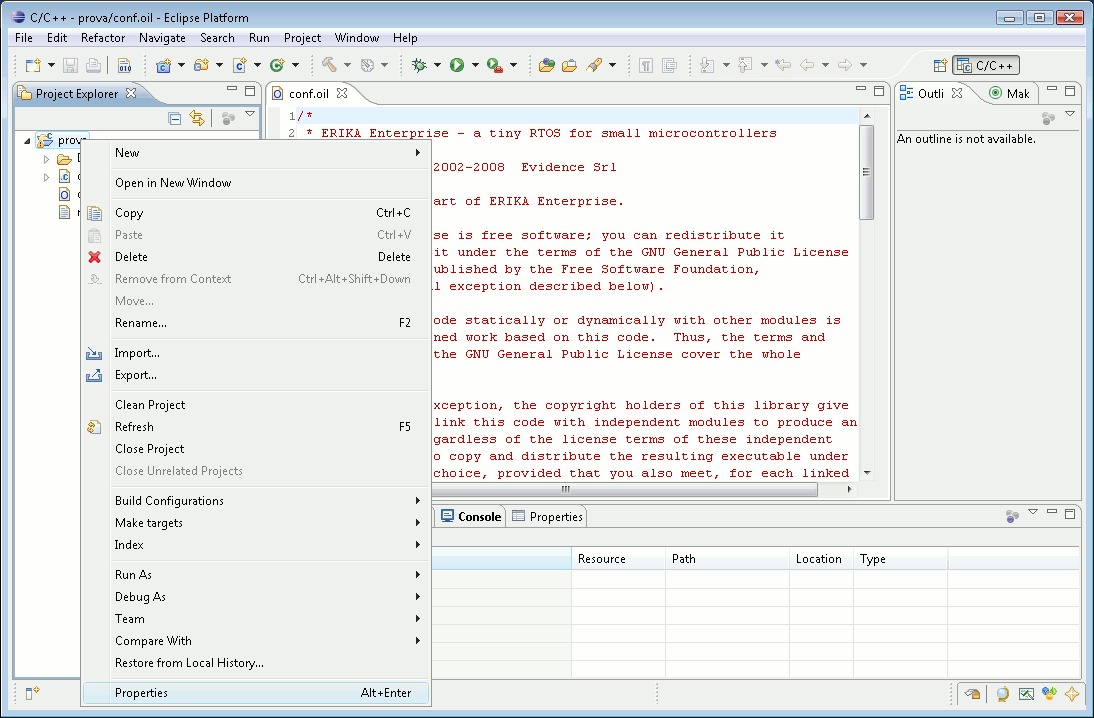
\includegraphics[width=6.3cm, bb=0 0 1094 718]{images/build1.png}
  \end{center}
  \caption{Opening the Project Properties.}
  \label{fig:build1}
\end{figure}

\begin{figure}
  \begin{center}
    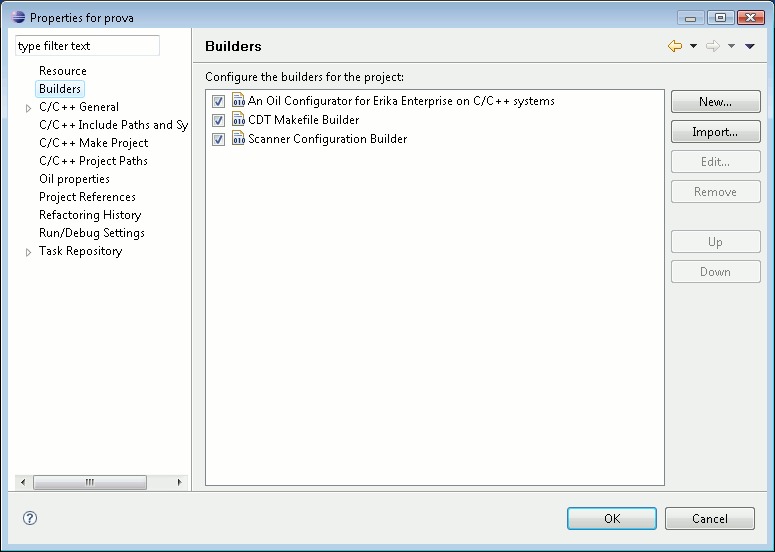
\includegraphics[width=6.3cm, bb=0 0 775 552]{images/build2.png}
  \end{center}
  \caption{The Builders property page. All checkboxes are selected by
    default.}
  \label{fig:build2}
\end{figure}

The first entry in Figure \ref{fig:build2} is relative to the \rtd\ 
Plugins shipped with Evidence, whereas the others are part of the CDT
\cite{Eclipse-CDT} plugin.




\section{Setting the OIL configuration file}

Whenever you need to set or change the OIL file that is used for code
generation, you must go to the ``Oil properties'' tab in the project
preference window. Open the Project Preference Window as shown in
Figure \ref{fig:build1}, then select the ``Oil properties'' item in
the left list, as shown in Figure \ref{fig:conf1}. After, you can type
the name of the Oil file in the ``File Name'' textbox, or you can
choose it by pressing the ``Browse'' button, as shown in Figure
\ref{fig:conf2}. The file {\em must} have a \file{.oil} extension.

\begin{figure}
  \begin{center}
    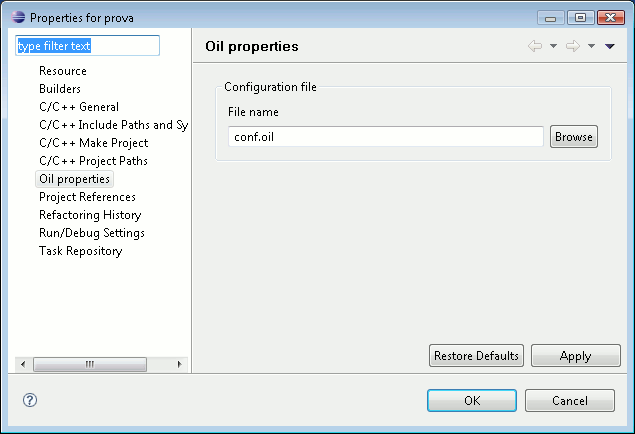
\includegraphics[width=6.2cm, bb=0 0 635 434]{images/conf1.png}
  \end{center}
  \caption{Changing the current OIL file for code generation.}
  \label{fig:conf1}
\end{figure}

\begin{figure}
  \begin{center}
    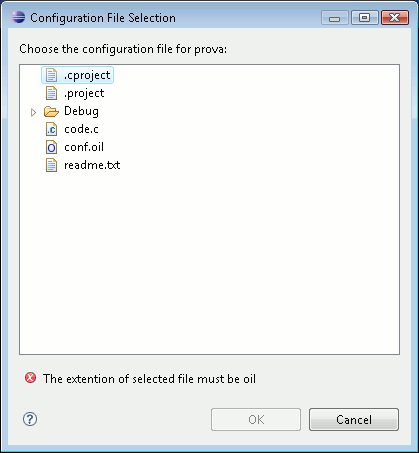
\includegraphics[width=3.5cm, bb=0 0 419 453]{images/conf2.png}
  \end{center}
  \caption{Choosing an existing OIL file by browsing the filesystem.}
  \label{fig:conf2}
\end{figure}





\section{Starting the Project Build procedure}

When the project Build is started, Eclipse executes the selected
builders. Figure \ref{fig:build2} shows the active Builders for a
project.

A project Build command can be run explicitly upon user request, or
automatically upon saving a file (see the option ``Build
Automatically'' in the ``Project'' menu). The manual execution of the
project Build command can be invoked by right clicking on the project
name in the navigation toolbar and then selecting ``Build Project'',
or directly from the ``Project'' menu, after having selected the
project in the navigation toolbar (see Figure
\ref{fig:buildproc1}).

\begin{figure}
  \begin{center}
    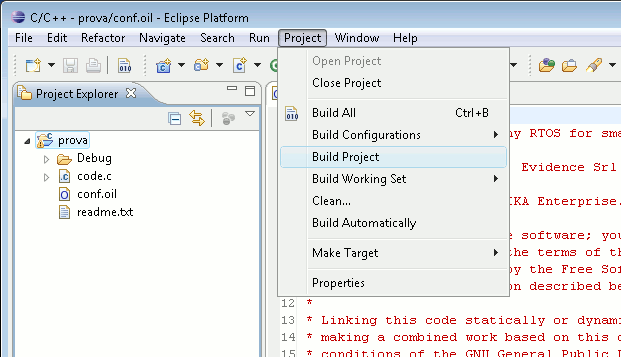
\includegraphics[width=4.4cm, bb=0 0 621 357]{images/buildproc1.png}
  \end{center}
  \caption{The ``Build Project'' option from the ``Project''
  menu. Please note that the ``Build Automatically'' option is not
  selected.}
  \label{fig:buildproc1}
\end{figure}

As a first step of the compilation process the \rtd\ builder is
launched. In this step the \rtd\ builder generates all the configuration 
scripts and the source code that is needed for the next steps of the
compilation process.

\begin{warning}
Be aware that when generating the code, the old build directories are
removed and completely overwritten!
\end{warning}

\rtd\ performs a code generation when one of the following conditions
apply:

\begin{itemize}
\item The OIL configuration file has been modified since the last
  build.
\item The Project properties have been modified, including the
  case in which the OIL configuration file name has been changed.
\item One or more files be generated do not exist anymore.
\item One or more files be generated is older than the OIL
configuration file.
\end{itemize}

The modification of the application source files does not imply
executing the \rtd\ code generation step.

The \rtd\ code generation is forced every time the OIL configuration 
file changes or the the project is cleaned as explained in Section 
\ref{project-clean}. 

After the \rtd\ builder generates the configuration source files and
scripts, the CDT builder is executed to compile the application. The
CDT Builder executes the make operation on the makefile that has been
generated by RT-Druid.

During the entire compilation phase, a progress window is displayed,
as shown in Figure \ref{fig:buildproc2}. The compilation can be done
in background by clicking on the ``Run in Background'' button in the
progress window.

\begin{figure}
  \begin{center}
    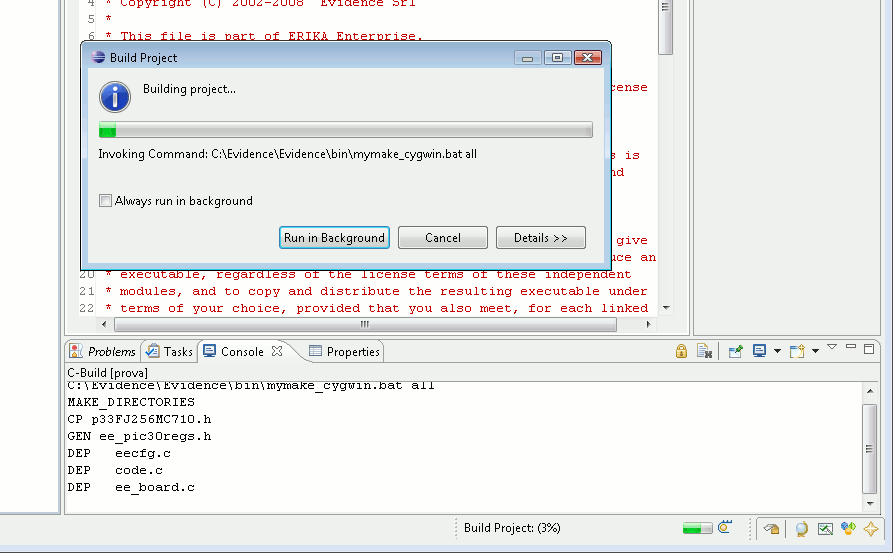
\includegraphics[width=5.1cm, bb=0 0 893 553]{images/buildproc2.png}
  \end{center}
  \caption{The Build progress window.}
  \label{fig:buildproc2}
\end{figure}

\section{RT-Druid Console}

Once the compilation process is completed, or if the compilation is
run in background, an \rtd\ console can be used to browse the messages
generated during code generation. To do that, the following steps must
be performed:

\begin{itemize}
\item Select the View ``console'' that typically appears in the 
  part of the screen after a build command.
\item Click on the monitor icon in the console view button list, and
  then choose ``RT-Druid output'' (see Figure \ref{fig:console1}).
\end{itemize}

\begin{figure}
  \begin{center}
    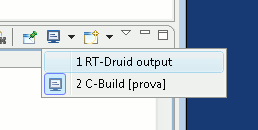
\includegraphics[width=2.3cm, bb=0 0 258 130]{images/console1.png}
  \end{center}
  \caption{Displaying the RT-Druid Console.}
  \label{fig:console1}
\end{figure}

As a result, a window like the one shown in Figure \ref{fig:console2}
appears. Please note that the text in the window can be selected and
copied as normal text.

\begin{figure}
  \begin{center}
    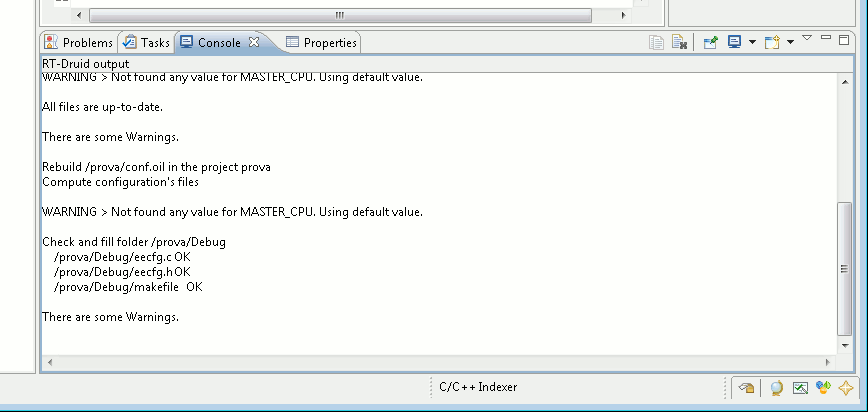
\includegraphics[width=7cm, bb=0 0 868 412]{images/console2.png}
  \end{center}
  \caption{The \rtd\ console.}
  \label{fig:console2}
\end{figure}

The pop-up menu in Figure \ref{fig:console2} can be obtained by right
clicking on the console. The menu allows to clear the content of the
console, to find strings inside it, or to drop the console\footnote{If
the console is dropped, a new one will appear at the next
build.}. Also note that upon a new build the new messages are appended
to the existing consoles.




\section{\ee\ Signatures}

The \ee\ kernel may be distributed in binary form. A so called
``binary distribution'' of \ee\ does not include the kernel C source
code, but only with a set of include files and precompiled
libraries. The \ee\ code is configured using \const{\#ifdef}
directives for efficiency reasons, and each library is the result of
the compilation of the \ee\ code with a specific combination of
\const{\#define}s.

The configurations used when generating the \ee\ libraries are
described in the \file{ee\\signature\\signature.xml} (for Altera Nios
II, the file is inside the \const{evidence_ee} SOPCBuilder component).

The location of the signature file is contained in the Eclipse
preferences, under the ``Windows/Preferences'' menu (see Figure
\ref{fig:sign1}). Then, inside the preferences Dialog box, select
``RT-Druid/Oil/OS Configurator'' (see Figure \ref{fig:sign2}).

\begin{figure}
  \begin{center}
    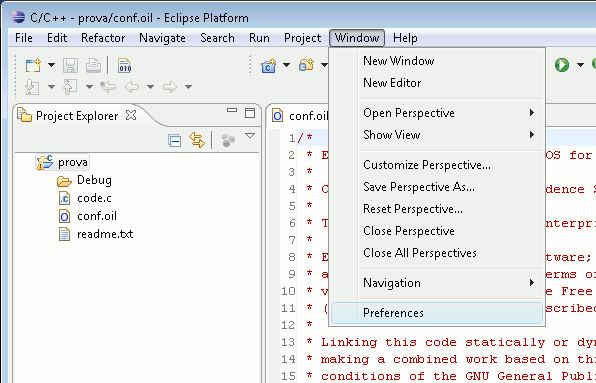
\includegraphics[width=4.6cm, bb=0 0 596 383]{images/sign1.png}
  \end{center}
  \caption{The ``Windows/Preferences'' menu item.}
  \label{fig:sign1}
\end{figure}

\begin{figure}
  \begin{center}
    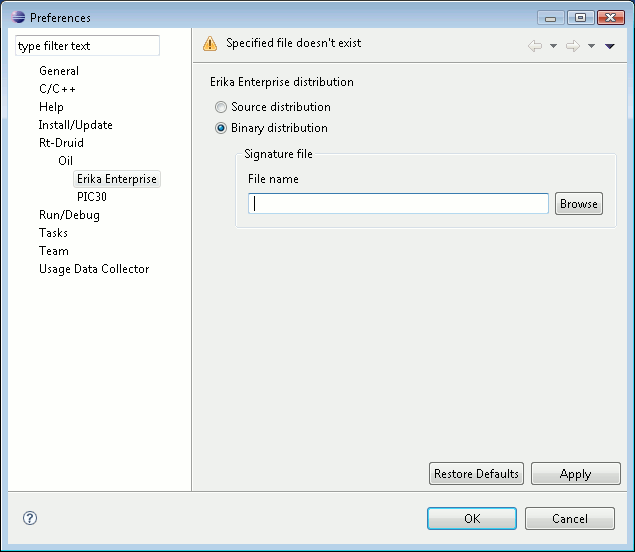
\includegraphics[width=7.3cm, bb=0 0 635 552]{images/sign2.png}
  \end{center}
  \caption{The OS Configurator dialog box.}
  \label{fig:sign2}
\end{figure}

In this box, the user can select if the code generator must be
configured for a source or for a binary distribution of \ee. When
using a Binary Distribution, the signature file location must be
specified. The standard location is ``Nios II Devices
Drivers/evidence\_ee/ee/signature/signature.xml'', as shown by Figure
\ref{fig:sign2}. Figure \ref{fig:sign4} shows the default location of
the \ee\ signatures.

If the system is correctly configured the signature file is
automatically found by \rtd\ without need of the user intervention.

\begin{figure}
  \begin{center}
    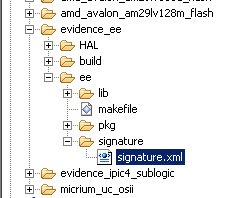
\includegraphics[width=2.4cm, bb=0 0 239 198]{images/sign4.png}
  \end{center}
  \caption{The default location of the signature file.}
  \label{fig:sign4}
\end{figure}

If \rtd\ is unable to find a library that can be used with the system
being generated, an error message is printed on the \rtd\ 
console, and the Build process is interrupted.

%\nb{(Mancano due immagini e da
%finire nel programma un mini HELP per capire come risolvere il
%problema)}

\section{Project cleanup}
\label{project-clean}

\rtd\  provides the feature to clean all the files produced by the code
generator. The cleanup process removes, if it
exists, the Build Directory.

To clean the project, just select the ``Clean...'' command inside the
``Project'' menu. The project need not be be selected if the command
is issued after selecting the project itself.

Please note the checkbox on the bottom left that can be used to build
the project right after the cleanup has been completed (see Figures
\ref{fig:clean2} and \ref{fig:clean2}).

\begin{figure}
  \begin{center}
    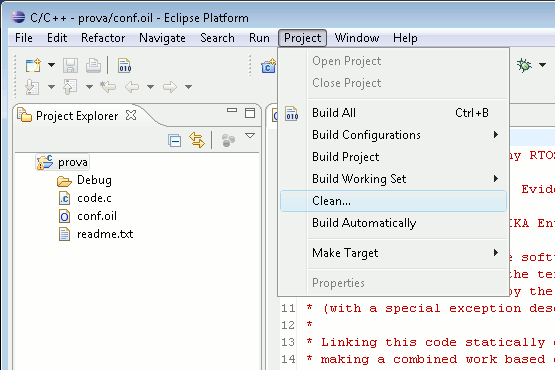
\includegraphics[width=4.4cm, bb=0 0 555 370]{images/clean1.png}
  \end{center}
  \caption{The ``Clean...'' command on the Project menu.}
  \label{fig:clean1}
\end{figure}

\begin{figure}
  \begin{center}
    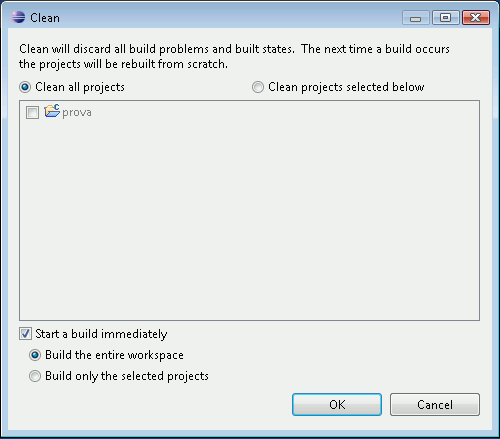
\includegraphics[width=5.3cm, bb=0 0 500 439]{images/clean2.png}
  \end{center}
  \caption{The Clean dialog box. Please note the bottom left checkbox.}
  \label{fig:clean2}
\end{figure}

Figures \ref{fig:clean3} and \ref{fig:clean4} shows the Navigation 
toolbar ``C/C++ projects'', before and after a project clean. The 
\file{Debug} directory have been removed, together with the ``Binary'' 
object list. During the cleanup, some errors may be shown in the Problem 
window. They can be ignored, since they refer to files that have been 
removed and that will be automatically re-created by \rtd\ at Build 
time. 

\begin{figure}
  \begin{center}
    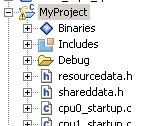
\includegraphics[width=1.6cm, bb=0 0 157 126]{images/clean3.png}
  \end{center}
  \caption{The Navigation toolbar before the Project clean.}
  \label{fig:clean3}
\end{figure}


\begin{figure}
  \begin{center}
    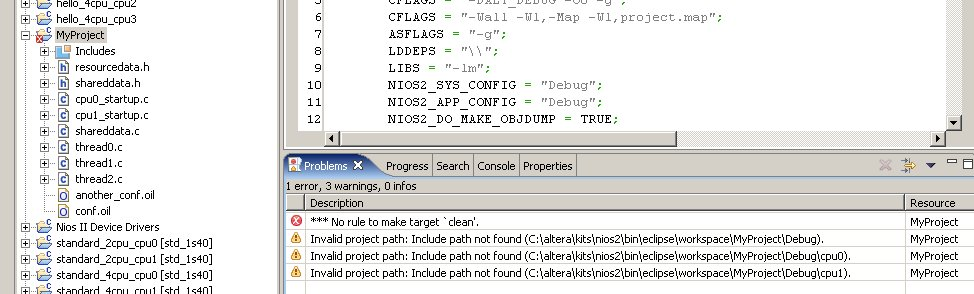
\includegraphics[width=9.8cm, bb=0 0 974 294]{images/clean4.png}
  \end{center}
  \caption{The Navigation toolbar after the Project clean. The errors
in the Problem window can be ignored, because they refer to files that
have been removed and that will be automatically created by \rtd\
at Build time.}
  \label{fig:clean4}
\end{figure}


\section{Application Debug and Run}
 
This section explicitly refers to the Altera Nios II target.

As a result of the compilation process, one ELF file for each CPU will
be placed inside the build directory. In the case of Altera Nios II,
these ELF files are equivalent to those built by traditional Altera
Build Scripts. To Debug and Run them, the best option is the creation
of a ``Multiprocessor collection'', as explained in the Altera
documentation \cite{Altera-multicpu-tutorial}.



\section{Application debug using Lauterbach Trace32}
\label{sec:trace32}

This section explicitly refers to the Altera Nios II target.

This section shows how to run a Lauterbach debug session using the
Trace32 scripts and ORTI files automatically generated by \rtd\ (see
Section \ref{sub:orti} for more information).

\begin{warning}
The scripts generated by \rtd\ suppose Lauterbach Trace32 being
installed in \file{C:\\t32}, and the Lauterbach ORTI utility
\file{genmenu.exe} being installed insie
\file{C:\\T32\\demo\\kernel\\orti}.
\end{warning}

Once the application has been compiled, and the Trace32 scripts have
been generated, launch Trace32 by double clicking on the
\file{Debug/debug.bat} file generated during the compilation. The
debugger opens up showing a window similar to the one in Figure
\ref{fig:trace32_splash}.

%
\begin{figure}
\begin{center}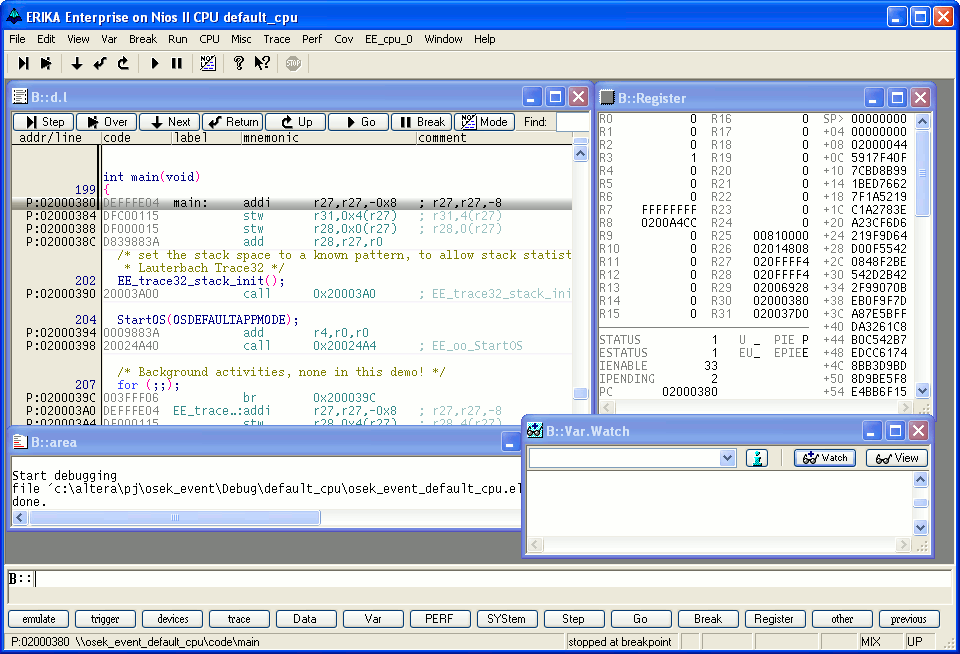
\includegraphics[%
  width=12cm, bb=0 0 960 654]{images/trace32_splash.png}\end{center}
\caption{\label{fig:trace32_splash} The Lauterbach Trace32 for Altera
Nios II.}
\end{figure}
%

Please note that each window has a title
with the name of the CPU being under debug. The menu list include a
submenu named ``ee\_cpu\_0'' containing the specification of the ORTI
related debug features.

By clicking on each menu item, you can get useful debug informations
about \ee. In particular:
\begin{itemize}
\item Figure \ref{fig:trace32_os} shows the general information about
  the kernel global variables, such as the name of the running task,
  the current priority of the running task, the last RTOS primitive
  called, the last error returned by an \ee\ primitive, the current
  application mode and the current system ceiling.
%
\begin{figure}
\begin{center}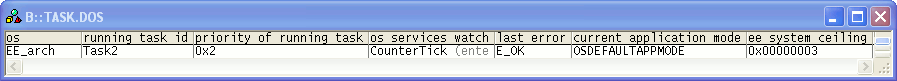
\includegraphics[%
  width=12cm, bb=0 0 897 81]{images/trace32_os.png}\end{center}
\caption{\label{fig:trace32_os} General information about the \ee\ status.}
\end{figure}
%

\item Figure \ref{fig:trace32_task} shows, for each task, the task
  name, its current priority, which may be different from the nominal
  priority when the task lock a resource, the task state, the task
  stack, and the current pending activations.
%
\begin{figure}
\begin{center}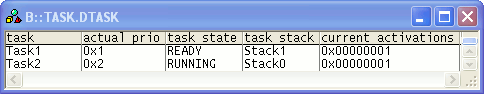
\includegraphics[%
  width=11cm, bb=0 0 484 94]{images/trace32_task.png}\end{center}
\caption{\label{fig:trace32_task} Information about the tasks in the
system.}
\end{figure}
%

\item Figure \ref{fig:trace32_resource} shows, for each resource, the
  resource name, the resource status, the task that has locked the
  resource (if any), and the ceiling priority of the resource.
%
\begin{figure}
\begin{center}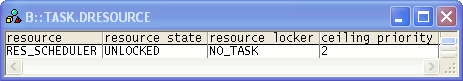
\includegraphics[%
  width=9cm, bb=0 0 463 81]{images/trace32_resource.png}\end{center}
\caption{\label{fig:trace32_resource} Information about the resources
in the system.}
\end{figure}
%

\item Figure \ref{fig:trace32_alarm} shows, for each alarm in the
  system, the alarm name, the time to which the alarm will fire, the
  cycle time of the alarm (\const{0x0} means the alarm is not cyclic),
  the alarm state, the action linked to the alarm notification, the
  counter to which the alarm is attached, and its value.
%
\begin{figure}
\begin{center}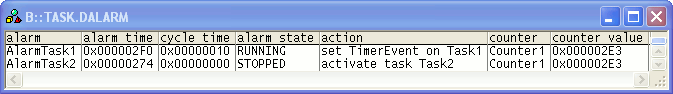
\includegraphics[%
  width=11cm, bb=0 0 673 94]{images/trace32_alarm.png}\end{center}
\caption{\label{fig:trace32_alarm} Information about the alarms in the
system.}
\end{figure}
%

\item Figure \ref{fig:trace32_stack} and Figure
  \ref{fig:trace32_stackview} show information about the stacks that
  has been configured in the application. In particular, the first
  figure shows the stack name, size, base address, direction, and fill
  pattern, while the second figure shows in a graphical way the
  current stack usage. To obtain the graphical stack usage estimation
  the application has to call \fn{EE_trace32_stack_init} at system
  startup. In this example, \const{Stack0} is the shared stack used by
  the background task (the \fn{main} function), and by
  \fn{Task2}. \fn{Stack1} is used by \fn{Task1}, and \fn{Stack2} is
  the interrupt stack.
%
\begin{figure}
\begin{center}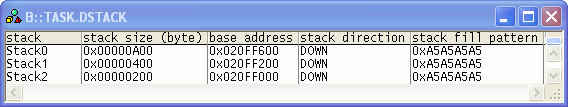
\includegraphics[%
  width=11cm, bb=0 0 568 107]{images/trace32_stack.png}\end{center}
\caption{\label{fig:trace32_stack} The application stack list.}
\end{figure}
%
\begin{figure}
\begin{center}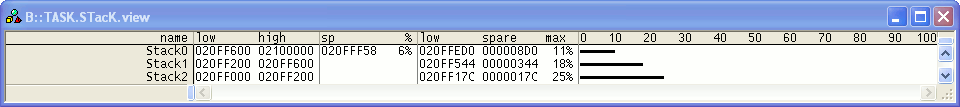
\includegraphics[%
  width=13cm, bb=0 0 960 107]{images/trace32_stackview.png}\end{center}
\caption{\label{fig:trace32_stackview} A graphical view of the
application stack usage.}
\end{figure}


\item Finally, whereas the previous figures were relative to the ORTI
  support provided for the \const{BCC1}, \const{BCC2}, \const{ECC1},
  \const{ECC2} kernels, Figure \ref{fig:trace32_frsh_orti} and Figure
  \ref{fig:trace32_frsh_task_graph} show the ORTI support for the
  \const{FRSH} kernel. In particular, the first figure shows the ORTI
  support for contracts, VRES, and budgets which are entities
  specifically introduced for the FRSH kernel, whereas the second
  figure shows the context changes as interpreted by Trace32
  considering the value changes of the running task pointer of the
  kernel logged using the Lauterbach tracer module.
%
\begin{figure}
\begin{center}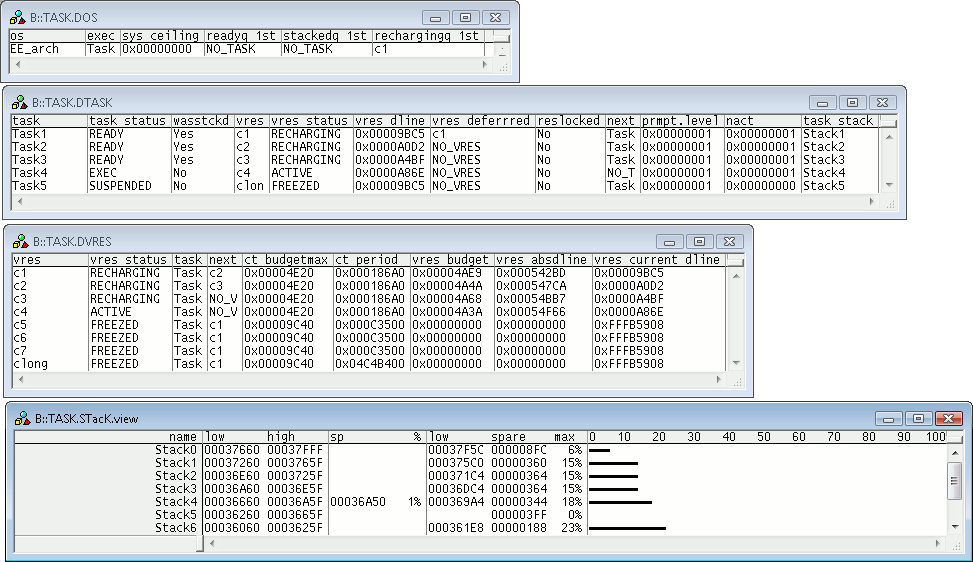
\includegraphics[%
  width=11cm, bb=0 0 973 562]{images/trace32_frsh_orti.png}\end{center}
\caption{\label{fig:trace32_frsh_orti} The ORTI windows for the FRSH Kernel.}
\end{figure}
%
\begin{figure}
\begin{center}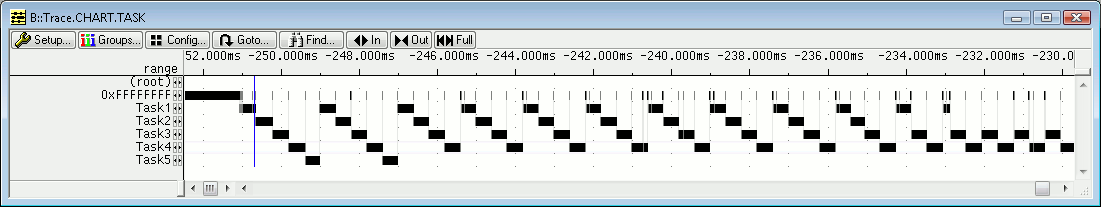
\includegraphics[%
  width=13cm, bb=0 0 1101 207]{images/trace32_fresh_task_graph.png}\end{center}
\caption{\label{fig:trace32_frsh_task_graph} An example of context change graphic produced by Lauterbach from the trace data of an application using the FRSH kernel.}
\end{figure}

\end{itemize}


The \rtd\ and \ee\ Trace32 support also includes support for the Nios
II tracer module. As an example, Figure \ref{fig:trace32_chart_irq}
shows the execution of an interrupt handler as recorded by the tracer
module. Figure \ref{fig:trace32_chart_state} shows an interpretation
of the context changes and task status values using the ORTI
information.

%
\begin{figure}
\begin{center}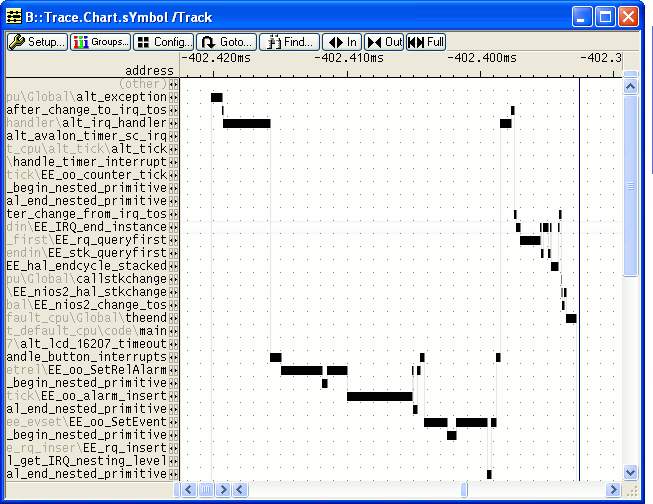
\includegraphics[%
  width=11cm, bb=0 0 653 504]{images/trace32_chart_irq.png}\end{center}
\caption{\label{fig:trace32_chart_irq} The execution of the Button IRQ
as recorded by Lauterbach Trace32.}
\end{figure}

%
\begin{figure}
\begin{center}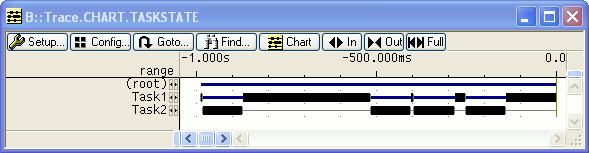
\includegraphics[%
  width=11cm, bb=0 0 589 153]{images/trace32_chart_state.png}\end{center}
\caption{\label{fig:trace32_chart_state} The interpretation of a trace
recorded with Lauterbach Trace32 showing the context changes happened
in the system.}
\end{figure}

\subsubsection{Acknowledgements}

We would like to thank Ing. Maurizio Menegotto from Lauterbach Italy
Srl for his support in the integration of \rtd\ and \ee\ with the
Lauterbach Trace32 Debugger and Tracer.

